\documentclass[11pt,a4paper]{report}

\usepackage[utf8]{inputenc}
\usepackage[portuges]{babel}
\usepackage{indentfirst}
\usepackage{graphicx}
\usepackage{float}
\usepackage{caption}
\usepackage{subcaption}
\usepackage[T1]{fontenc}
\usepackage{listings}
\usepackage{amsmath}
\usepackage{mathtools}
\usepackage{tikz}
\renewcommand{\familydefault}{\sfdefault}

% packages que adicionei do stor
\usepackage{xspace}
\setlength{\oddsidemargin}{-1cm}
\setlength{\textwidth}{18cm}
\setlength{\headsep}{-1cm}
\setlength{\textheight}{23cm}

\title{Processamento de Linguagens (3º ano de Curso)\\
	\textbf{Trabalho Prático Nº1}\\ Relatório de Desenvolvimento}
\author{Diogo Braga\\ A82547 \and João Silva\\ A82005 \and Ricardo Caçador\\ A81064}
\date{\today}

\begin{document}

\maketitle

\begin{abstract}
	Neste relatório é apresentada a resolução de um exercício referente ao TP1, que tem como objetivos a utilização de Expressões Regulares para descrição de padrões de frases, e a utilização do Flex para gerar filtros de texto em C.
Outro objetivo será ainda desenvolver, a partir de ERs, sistemática e automaticamente Processadores de Linguagens Regulares, que filtrem ou transformem textos com base no conceito de regras de produção Condição-Ação.
\end{abstract}

\tableofcontents

\newpage

\chapter{Introdução}
\label{chap:intro}

Seguindo a fórmula \emph{exe= (N\_Alu\% 7) + 1} e o número de aluno mais baixo presente no nosso grupo (81064), o enunciado correspondente é o \textbf{5 - WikiQuotes: provérbios}.

Este enunciado apresenta-nos um tema relacionado com várias citações de vários autores, vários provérbios de línguas diferentes, e ainda provérbios que são variações dos originais e alguns que são adulterações dos originais. Este tipo de material está armazenado num ficheiro \emph{XML}, onde se encontra muitas vezes organizado e outras vezes não tão bem organizado.

Ao longo deste trabalho produzimos essencialmente 3 filtros cada um com um objetivo bem delimitado. O primeiro filtro atua sobre as citações contidas em páginas de autor, o segundo filtro retém todas as citações cujo título da página comece com "Provérbios" e, por último, o terceiro filtro procura um padrão de provérbios que estejam adulterados. Neste último caso optamos também por filtrar os provérbios que são variações. De referir ainda que ligamos os provérbios adulterados e os que são variações ao respetivo provérbio original. O pergunta 4 do enunciado, o grupo optou por não a fazer separadamente dos outros filtros pelos que cada filtro apresenta estatísticas sobre o seu trabalho.

Com este relatório pretendemos apresentar as nossas opções, algoritmos desenvolvidos e ainda estruturas utilizadas para a realização de cada filtro. Pretendemos também apoiar aquelas que foram as nossas soluções, com conhecimento obtido nas aulas teóricas, relembrando por exemplo o caso dos autómatos.

Para uma melhor visão do que irá ser abordado neste relatório deixamos uma breve descrição daquilo que foi feito. No segundo capítulo foi feita uma análise informal e uma especificação dos requisitos deste projeto. No terceiro capítulo foi realizado o desenho da conceção no qual estão envolvidos os algoritmos e estruturas de dados usados. No quarto capítulo mostramos alguns exemplos de implementações e vários resultados de testes realizados. Por último no capítulo 5 fazemos uma retrospetiva do trabalho realizado e concluímos.



\chapter{Análise e Especificação}
\label{chap:analise}

Analisando o problema como um todo o que podemos encontrar aquando da observação do ficheiro \textbf{ptwikiquote-20190301-pages-articles.xml}, são várias meticulosidades no que toca à organização das páginas, títulos, citações, provérbios, etc. Contudo o nosso objetivo central é filtrar somente o que achamos necessário para respeitar os requisitos impostos pelo enunciado e descritos nas subsecções seguintes.

Nas secções seguintes serão apresentados os objetivos de cada alínea do exercício e ainda as observações que foram feitas ao ficheiro que contém todo o \emph{XML}, por forma a pensar que casos iríamos ter futuramente e começarmos a delinear uma arquitetura duma possível solução.

\section{Análise e Especificação dos Requisitos}
\subsection{Lista de Citações}

Na primeira alínea do exercício, era requerido um filtro que criasse uma lista de citações com o respetivo autor, somente se estas citações se encontrarem numa página de autor.

Ao proceder à análise do ficheiro \emph{XML} reparamos que uma página seria de autor se contivesse o seguinte cenário dentro da mesma:

\begin{figure}[H]
\centering
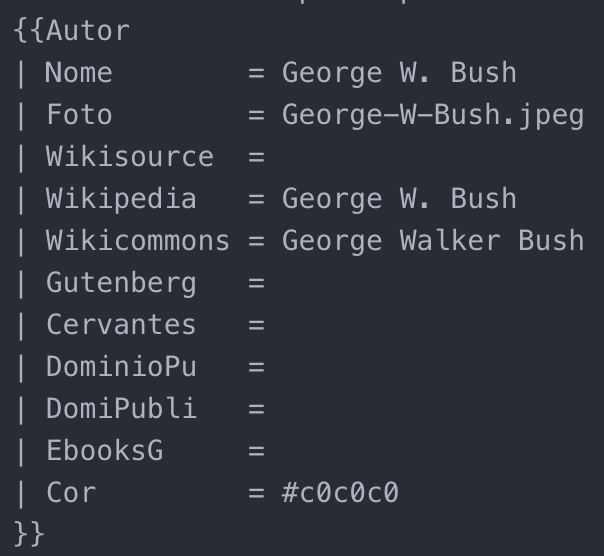
\includegraphics[scale=0.75]{pagina_autor.png}
\caption{Estrutura descritiva de um autor.}
\label{img:pagina_autor}
\end{figure}

Obviamente existem páginas que contém informações mais volumosas sobre um autor e outras páginas que contém menos. Posto isto reparamos que o campo \textbf{Nome}, pode ou não estar preenchido. Para os casos em que não está preenchido, o grupo achou por bem não considerar que a página se trataria de um autor, ignorando todos as citações na página contidas. O campo \textbf{Nome} possuía ainda outro pormenor. Muitas vezes surge referenciado noutra língua como por exemplo espanhol (\emph{Nombre}) e inglês (\emph{Name}).

Em páginas de autor investigámos de que forma aparecem a maior parte das citações que estes fazem. Chegamos à conclusão que na maior parte dos casos as citações surgem da seguinte forma:

\begin{figure}[H]
\centering
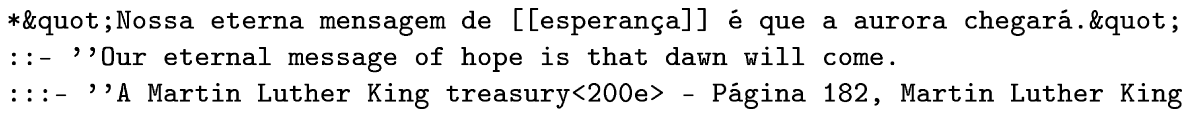
\includegraphics[scale=0.75]{quote.png}
\caption{Estrutura duma citação.}
\label{img:quote}
\end{figure}

Conseguimos identificar que a maior parte das citações de autores se encontram no meio de \textbf{\&quot;} e apenas teríamos de filtrar o que estivesse entre duas marcas deste tipo. Mas com a análise de mais casos deparámo-nos com situações desta natureza:

\begin{figure}[H]
\centering
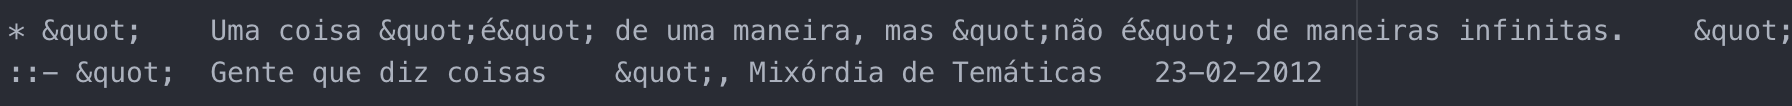
\includegraphics[scale=0.6]{marca_dentro_quote.png}
\caption{Exemplo de quatro marcas dentro duma citação.}
\label{img:marca_in_quote}
\end{figure}

Contudo surgiram muitos mais casos durante esta análise podemos referir casos em que citações não terminam com a marca \textbf{\&quot;} mas em vez disso acabam com por exemplo \textbf{::-}, ou \textbf{:-}, e ainda \textbf{**}.

Estes casos e muitos mais serão tratados nos capítulos seguintes.


\newpage

\subsection{Lista de Provérbios}
\label{subsec:analise2}

Nesta segunda alínea do exercício, era requerido um filtro que criasse uma lista de provérbios (citações contidas em páginas cujo título começa por "Provérbios").

Procedendo à análise do ficheiro \textit{XML} foi possível entender a forma como se organiza a informação nas páginas que referem provérbios:

\begin{figure}[H]
\centering
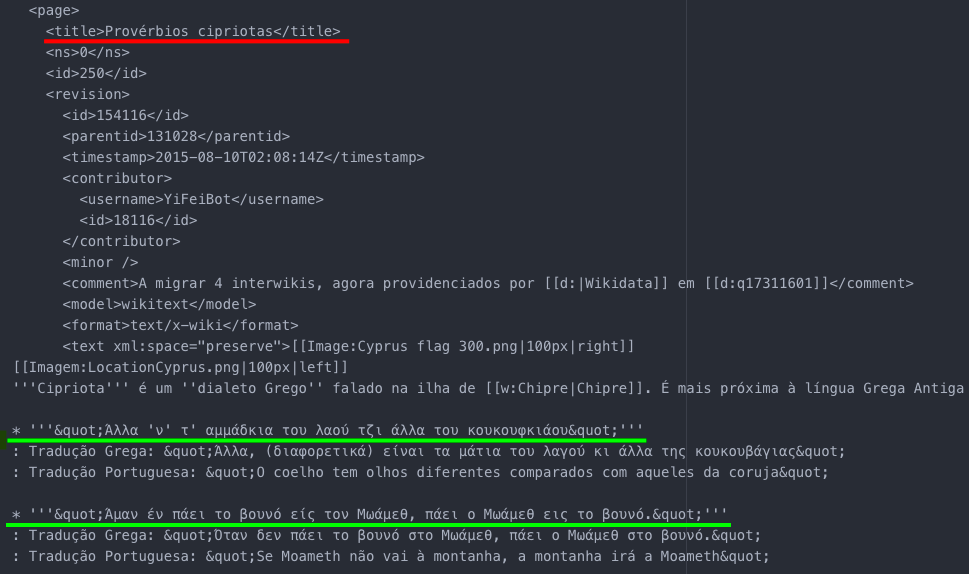
\includegraphics[scale=0.45]{pagina_titulo.png}
\caption{Exemplo de uma página de provérbios.}
\label{img:pagina_titulo}
\end{figure}

Neste caso, está exemplificada a página na qual o título é \textbf{Provérbios cipriotas}, visto que este se encontra entre as marcas \underline{<title>} e \underline{</title>}. É, portanto, desta forma que são identificadas as páginas que temos interesse em aceder. Tal facto aparece sublinhado a vermelho na figura.

Aquando da análise do ficheiro foram encontrados casos em que o título continha a palavra "Provérbio", mas não era inicializado por esta. É importante, de facto, ter em conta este caso pois tal é requirido no enunciado do exercício.

Filtrando os títulos das páginas, procuramos saber quais as marcas que indicam o início de um provérbio. Neste caso, sublinhado a verde, é possível concluir que a marca de início é \underline{* '''\&quot;} , enquanto a marca de fim é \underline{\&quot;'''}.

Realizada a análise das páginas de provérbios, foi possível concluir que existem inúmeras formas de identificar o início e o fim dum provérbio. Tal acontece porque o ficheiro contém muita variedade de idiomas e, consequentemente, diferentes ideias das diferentes pessoas que decidem quais as marcas a usar nas citações.

	\vspace{0.2cm}

Alguns exemplos de marcas de início de provérbios presentes no ficheiro são:
\begin{itemize}
 \item *\&quot;
 \item *\&quot;''
 \item **''\&quot;
 \item :'''
\end{itemize}

	\vspace{0.2cm}

Por outro lado, alguns exemplos de marcas de final de provérbios presentes no ficheiro são:
\begin{itemize}
 \item \&quot;
 \item \&quot;''
 \item ''\&quot;
 \item '''
\end{itemize}

	\vspace{0.2cm}

A ideia inicial foi generalizar as expressões regulares para qualquer página de provérbios, mas devido ao facto de existirem inúmeras marcas diversificadas foi necessário criar alguns contextos específicos para cada país, de forma a que não houvessem conflitos entre marcas e fosse possível criar um output perceptível.

Nos capítulos seguintes serão abordados pormenorizadamente estes casos.


\subsection{Lista de Provérbios Adulterados}

Nesta terceira alínea do exercício, era requerida a listagem dos provérbios "adulterados" e o seu original. Era suposto procurar um padrão que identificasse estes provérbios.

Ao proceder à análise do ficheiro \textit{XML} foi possível concluir que os provérbios adulterados e alternativos seriam apresentados da seguinte forma:

\begin{figure}[H]
\centering
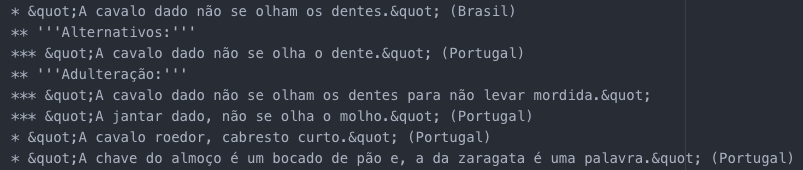
\includegraphics[scale=0.60]{pagina_adulterados.png}
\caption{Exemplo de uma página com provérbios adulterados e alternativos.}
\label{img:pagina_adulterados}
\end{figure}

A seleção das páginas a filtrar é realizada tal como na subsecção \ref{subsec:analise2}, isto é, selecionamos as páginas cujo título começa por "Provérbios". Tendo em conta este requisito, o filtro a seguir é também aplicado ao que se encontra entre as marcas \underline{<title>} e \underline{</title>} duma página.

Filtrando os títulos das páginas, procuramos depois saber quais as marcas que indicam um provérbio adulterado e um provérbio alternativo. Importante referir que decidimos tomar como diferentes estas qualificações.

\vspace{0.2cm}

Segundo a nossa análise, a indicação de provérbios adulterados/alternativos acontece, em regra geral, da seguinte forma:
\begin{enumerate}
\item É apresentado um provérbio inicializado com a marca \underline{* \&quot;} e finalizado com a marca \underline{\&quot;} ;
	\begin{enumerate}
		\item Caso a linha seguinte seja inicializada da mesma forma, o provérbio não contém adulterações;
	\end{enumerate}
\item É apresentada a marca \underline{** '''Alternativos:'''}, ou \underline{** '''Adulteração:'''} ou \underline{** '''Adulterados:'''}, que mostra que a seguir vão ser listados esses provérbios;
	\begin{enumerate}
		\item Caso seja \underline{** '''Alternativos:'''}, é inicializada a fase dos provérbios alternativos;
		\item Caso seja \underline{** '''Adulteração:'''} ou \underline{** '''Adulterados:'''}, é inicializada a fase dos provérbios adulterados;
	\end{enumerate}
\item É apresentado um provérbio inicializado com a marca \underline{*** \&quot;} e finalizado com a marca \underline{\&quot;} , que é o alternativo ou o adulterado da citação apresentada no passo 1.
\end{enumerate}

\vspace{0.2cm}

Na figura \ref{img:pagina_adulterados}, é possível visualizar um caso destes:

\begin{itemize}
\item Provérbio original que contém adulterações $\Rightarrow$ "A cavalo dado não se olham os dentes."
\item Provérbio alternativo $\Rightarrow$ "A cavalo dado não se olha o dente."
\item Provérbio adulterado 1 $\Rightarrow$ "A cavalo dado não se olham os dentes para não levar mordida."
\item Provérbio adulterado 2 $\Rightarrow$ "A jantar dado, não se olha o molho."
\item Provérbio sem adulterações $\Rightarrow$ "A cavalo roedor, cabresto curto"
\item Provérbio indefenido (depende do que aparecer na linha seguinte) $\Rightarrow$ "A chave do almoço é um bocado de pão e, a da zaragata é uma palavra."
\end{itemize}

\vspace{0.2cm}

Existe também a possibilidade de um provérbio ter só adulterados ou só alternativos. Todos estes casos serão abordados nos capítulos seguintes.

\subsection{Estatísticas dos elementos encontrados}

Nesta quarta alínea do exercício, era requerida a apresentação de estatísticas referentes ao que foi filtrado nas alíneas anteriores.

Importante referir que o grupo tomou a decisão de apresentar tais resultados individualmente nas questões ao invés de tudo nesta parte. Esta decisão assim aconteceu porque achamos mais benéfico saber as estatísticas dos resultados em cada questão, visto ser mais fácil a sua análise.





\chapter{Concepção/desenho da Resolução}
\label{chap:concepcao}

\section{Algoritmos}
\subsection{Lista de Citações}

\begin{center}
\begin{tikzpicture}[scale=0.2]
\tikzstyle{every node}+=[inner sep=0pt]
\draw [black] (9.2,-21.5) circle (3);
\draw (9.2,-21.5) node {$INITIAL$};
\draw [black] (31.7,-21.5) circle (3);
\draw (31.7,-21.5) node {$PAGE$};
\draw [black] (50.8,-21.5) circle (3);
\draw (50.8,-21.5) node {$AUTOR$};
\draw [black] (71.9,-21.5) circle (3);
\draw (71.9,-21.5) node {$QUOTE$};
\draw [black] (50.1,-39.8) circle (3);
\draw (50.1,-39.8) node {$NOME\_AUTOR$};
\draw [black] (1.6,-21.5) -- (6.2,-21.5);
\fill [black] (6.2,-21.5) -- (5.4,-21) -- (5.4,-22);
\draw [black] (28.805,-22.285) arc (-77.1203:-102.8797:37.484);
\fill [black] (28.81,-22.28) -- (27.91,-21.98) -- (28.14,-22.95);
\draw (20.45,-23.73) node [below] {$nova\_pagina$};
\draw [black] (34.7,-21.5) -- (47.8,-21.5);
\fill [black] (47.8,-21.5) -- (47,-21) -- (47,-22);
\draw (41.25,-22) node [below] {$inicio\_autor$};
\draw [black] (48.57,-37.226) arc (-155.15368:-209.22747:14.613);
\fill [black] (48.57,-37.23) -- (48.69,-36.29) -- (47.78,-36.71);
\draw (46.67,-30.51) node [left] {$nome\_autor$};
\draw [black] (52.324,-24.078) arc (24.73681:-29.11795:14.66);
\fill [black] (52.32,-24.08) -- (52.21,-25.01) -- (53.11,-24.6);
\draw (54.22,-30.79) node [right] {$nome\mbox{ }>\mbox{ }1$};
\draw [black] (47.272,-40.784) arc (-77.04436:-192.6434:13.785);
\fill [black] (30.73,-24.33) -- (30.07,-25) -- (31.04,-25.22);
\draw (29.84,-37.6) node [below] {$nome\mbox{ }=\mbox{ }"\ "$};
\draw [black] (68.978,-22.175) arc (-79.12516:-100.87484:40.429);
\fill [black] (68.98,-22.17) -- (68.1,-21.83) -- (68.29,-22.82);
\draw (61.35,-23.4) node [below] {$\*quote\_token$};
\draw [black] (53.54,-20.284) arc (110.13881:69.86119:22.683);
\fill [black] (53.54,-20.28) -- (54.46,-20.48) -- (54.12,-19.54);
\draw (61.35,-18.4) node [above] {$fim\_quote$};
\draw [black] (7.59,-18.983) arc (240.34019:-47.65981:2.25);
\draw (7.32,-13.86) node [above] {$fim\_pagina$};
\fill [black] (10.22,-18.69) -- (11.05,-18.24) -- (10.18,-17.75);
\draw [black] (12.075,-20.647) arc (104.02759:75.97241:34.551);
\fill [black] (12.08,-20.65) -- (12.97,-20.94) -- (12.73,-19.97);
\draw (20.45,-19.12) node [above] {$fim\_pagina$};
\draw [black] (11.541,-19.626) arc (125.94601:54.05399:31.445);
\fill [black] (11.54,-19.63) -- (12.48,-19.56) -- (11.9,-18.75);
\draw (30,-13.14) node [above] {$fim\_pagina$};
\draw [black] (10.875,-19.012) arc (143.70718:36.29282:36.817);
\fill [black] (10.88,-19.01) -- (11.75,-18.66) -- (10.95,-18.07);
\draw (40.55,-3.49) node [above] {$fim\_pagina$};
\end{tikzpicture}
\end{center}


\underline{Definições: }
\begin{itemize}
	\item espacos $\Rightarrow$ [\ ]*
	\item nova\_pag $\Rightarrow$ <page>
	\item fim\_pag $\Rightarrow$ </page>
	\item nome\_linguas $\Rightarrow$ (Nome|Nombre|Name)
	\item inicio\_autor $\Rightarrow$ \{\{(?i:Autor)
	\item fim\_autor $\Rightarrow$ \}\}
	\item nome\_autor $\Rightarrow$ |\{espacos\}\{nome\_linguas\}\{espacos\}=\{espacos\}
	\item quote\_token $\Rightarrow$ \{espacos\}\&quot;
\end{itemize}

\vspace{0.5cm}

\textbf{Definição do autómato:}

\begin{itemize}
	\item Estados do autómato:
		\begin{itemize}
			\item INITIAL
			\item PAGE
			\item AUTOR
			\item NOME\_AUTOR
			\item QUOTE
		\end{itemize}
	\item Estado inicial:
		\begin{itemize}
			\item INITIAL
		\end{itemize}
	\item Estados finais:  ---
	\item Funções de Transição:
\end{itemize}



\newpage

\subsection{Lista de Provérbios}

\begin{center}
\begin{tikzpicture}[scale=0.2]
\tikzstyle{every node}+=[inner sep=0pt]
\draw [black] (9.9,-32.9) circle (3);
\draw (9.9,-32.9) node {$INIT$};
\draw [black] (26.9,-32.9) circle (3);
\draw (26.9,-32.9) node {$PAGE$};
\draw [black] (57.8,-32.9) circle (3);
\draw (57.8,-32.9) node {$PC$};
\draw [black] (75.3,-32.9) circle (3);
\draw (75.3,-32.9) node {$Q$};
\draw [black] (12.9,-32.9) -- (23.9,-32.9);
\fill [black] (23.9,-32.9) -- (23.1,-32.4) -- (23.1,-33.4);
\draw (18.4,-33.4) node [below] {$nova\_pag$};
\draw [black] (12.016,-30.787) arc (126.88455:53.11545:10.637);
\fill [black] (12.02,-30.79) -- (12.96,-30.71) -- (12.36,-29.91);
\draw (18.4,-28.16) node [above] {$fim\_pag$};
\draw [black] (29.9,-32.9) -- (54.8,-32.9);
\fill [black] (54.8,-32.9) -- (54,-32.4) -- (54,-33.4);
\draw (42.35,-32.4) node [above] {$ini\_titProverbios.*fim\_tit$};
\draw [black] (72.378,-33.574) arc (-79.65641:-100.34359:32.458);
\fill [black] (72.38,-33.57) -- (71.5,-33.23) -- (71.68,-34.21);
\draw (66.55,-34.6) node [below] {$inicio\_quote$};
\draw [black] (60.641,-31.942) arc (104.90535:75.09465:22.974);
\fill [black] (60.64,-31.94) -- (61.54,-32.22) -- (61.28,-31.25);
\draw (66.55,-30.67) node [above] {$fim\_quote$};
\draw [black] (2.1,-32.9) -- (6.9,-32.9);
\fill [black] (6.9,-32.9) -- (6.1,-32.4) -- (6.1,-33.4);
\draw [black] (11.519,-30.375) arc (145.07326:34.92674:37.91);
\fill [black] (11.52,-30.37) -- (12.39,-30.01) -- (11.57,-29.43);
\draw (42.6,-13.67) node [above] {$fim\_pag$};
\draw [black] (11.598,-30.429) arc (142.43928:37.56072:28.07);
\fill [black] (11.6,-30.43) -- (12.48,-30.1) -- (11.69,-29.49);
\draw (33.85,-18.97) node [above] {$fim\_pag$};
\end{tikzpicture}
\end{center}

\underline{Nota:} -

	\vspace{1.0cm}

\textbf{Definições: }
\begin{itemize}
	\item -
\end{itemize}

	\vspace{1.0cm}

\textbf{Definição do autómato:}

\begin{itemize}
	\item Estados do autómato:
		\begin{itemize}
			\item -
		\end{itemize}
	\item Estado inicial: INIT
	\item Estados finais: ---
	\item Funções de Transição:
		\begin{itemize}
			\item -
		\end{itemize}
\end{itemize}




\newpage

\subsection{Lista de Provérbios Adulterados}

\begin{center}
\begin{tikzpicture}[scale=0.2]
\tikzstyle{every node}+=[inner sep=0pt]
\draw [black] (8.9,-4.7) circle (3);
\draw (8.9,-4.7) node {$INIT$};
\draw [black] (25.8,-4.7) circle (3);
\draw (25.8,-4.7) node {$PAGE$};
\draw [black] (57.8,-4.7) circle (3);
\draw (57.8,-4.7) node {$PC$};
\draw [black] (40.4,-18.5) circle (3);
\draw (40.4,-18.5) node {$Q$};
\draw [black] (40.4,-29.9) circle (3);
\draw (40.4,-29.9) node {$QC$};
\draw [black] (17.1,-38.6) circle (3);
\draw (17.1,-38.6) node {$ADU$};
\draw [black] (63.3,-38.6) circle (3);
\draw (63.3,-38.6) node {$ALT$};
\draw [black] (17.1,-56.4) circle (3);
\draw (17.1,-56.4) node {$QADU$};
\draw [black] (63.3,-56.4) circle (3);
\draw (63.3,-56.4) node {$QALT$};
\draw [black] (10.223,-7.38) arc (54:-234:2.25);
\draw (8.9,-11.95) node [below] {$fim\_pag$};
\fill [black] (7.58,-7.38) -- (6.7,-7.73) -- (7.51,-8.32);
\draw [black] (11.9,-4.7) -- (22.8,-4.7);
\fill [black] (22.8,-4.7) -- (22,-4.2) -- (22,-5.2);
\draw (17.35,-5.2) node [below] {$nova\_pag$};
\draw [black] (2.1,-4.7) -- (5.9,-4.7);
\fill [black] (5.9,-4.7) -- (5.1,-4.2) -- (5.1,-5.2);
\draw [black] (28.8,-4.7) -- (54.8,-4.7);
\fill [black] (54.8,-4.7) -- (54,-4.2) -- (54,-5.2);
\draw (41.8,-5.2) node [below] {$ini\_tit$Proverbios.*$fim\_tit$};
\draw [black] (55.45,-6.56) -- (42.75,-16.64);
\fill [black] (42.75,-16.64) -- (43.69,-16.53) -- (43.07,-15.75);
\draw (55.33,-12.1) node [below] {$*quote\_token$};
\draw [black] (39.563,-27.024) arc (-169.37552:-190.62448:15.318);
\fill [black] (39.56,-27.02) -- (39.91,-26.15) -- (38.92,-26.33);
\draw (38.8,-24.2) node [left] {.*$quote\_token$};
\draw [black] (37.697,-31.201) arc (-65.0152:-74.03449:120.165);
\fill [black] (19.99,-37.81) -- (20.9,-38.07) -- (20.63,-37.11);
\draw (35.41,-35.52) node [below] {$**adulterados$};
\draw [black] (43.398,-29.835) arc (88.28203:50.11313:28.961);
\fill [black] (61.1,-36.56) -- (60.81,-35.66) -- (60.17,-36.43);
\draw (59.34,-31.05) node [above] {$**alternativos$};
\draw [black] (19.719,-37.137) arc (118.00528:102.94504:72.268);
\fill [black] (19.72,-37.14) -- (20.66,-37.2) -- (20.19,-36.32);
\draw (21.94,-32.57) node [above] {$**adulteracao$};
\draw [black] (17.156,-35.604) arc (-185.50339:-272.93049:19.371);
\fill [black] (37.43,-18.12) -- (36.65,-17.58) -- (36.6,-18.57);
\draw (17.55,-22.3) node [above] {$*quote\_token$};
\draw [black] (16.426,-53.478) arc (-169.60117:-190.39883:33.118);
\fill [black] (16.43,-53.48) -- (16.77,-52.6) -- (15.79,-52.78);
\draw (15.38,-47.5) node [left] {$***quote\_token$};
\draw [black] (62.681,-53.466) arc (-170.46728:-189.53272:36.021);
\fill [black] (62.68,-53.47) -- (63.04,-52.59) -- (62.06,-52.76);
\draw (61.68,-47.5) node [left] {$***quote\_token$};
\draw [black] (43.381,-18.188) arc (91.55223:5.89903:19.419);
\fill [black] (43.38,-18.19) -- (44.19,-18.67) -- (44.17,-17.67);
\draw (62.95,-22.52) node [above] {$*quote\_token$};
\draw [black] (60.305,-38.77) arc (-86.97892:-93.02108:381.471);
\fill [black] (20.1,-38.77) -- (20.87,-39.31) -- (20.92,-38.31);
\draw (40.2,-39.8) node [below] {$**adulterados$};
\draw [black] (60.532,-39.755) arc (-68.8716:-111.1284:56.405);
\fill [black] (19.87,-39.76) -- (20.43,-40.51) -- (20.79,-39.58);
\draw (40.2,-44.05) node [below] {$**adulteracao$};
\draw [black] (17.873,-41.497) arc (11.97339:-11.97339:28.935);
\fill [black] (17.87,-41.5) -- (17.55,-42.38) -- (18.53,-42.18);
\draw (19,-47.5) node [right] {.*$quote\_token$};
\draw [black] (64.243,-41.446) arc (14.72619:-14.72619:23.817);
\fill [black] (64.24,-41.45) -- (63.96,-42.35) -- (64.93,-42.09);
\draw (65.53,-47.5) node [right] {.*$quote\_token$};
\draw [black] (41.089,-21.416) arc (8.65405:-8.65405:18.5);
\fill [black] (41.09,-21.42) -- (40.72,-22.28) -- (41.7,-22.13);
\draw (41.8,-24.2) node [right] {$*quote\_token$};
\end{tikzpicture}
\end{center}

\underline{Nota:} Todos os estados do autômato possuem uma condição \textit{fim\_pag} para o estado INIT. Neste autômato só está representado no próprio estado INIT.

	\vspace{1.0cm}

\textbf{Definições: }
\begin{itemize}
	\item espacos $\Rightarrow$ [\ ]*
	\item nova\_pag $\Rightarrow$ <page>
	\item fim\_pag $\Rightarrow$ </page>
	\item ini\_tit $\Rightarrow$ <title>
	\item fim\_tit $\Rightarrow$ </title>
	\item quote\_token $\Rightarrow$ \{espacos\}\&quot;\{espacos\}
	\item adulteracao $\Rightarrow$ \{espacos\}'''Adulteração:'''
	\item alternativos $\Rightarrow$ \{espacos\}'''Alternativos:'''
	\item adulterados $\Rightarrow$ \{espacos\}'''Adulterados:'''
\end{itemize}

	\vspace{1.0cm}

\textbf{Definição do autómato:}

\begin{itemize}
	\item Estados do autómato:
		\begin{itemize}
			\item INIT $\Rightarrow$ INITIAL
			\item PAGE
			\item PC $\Rightarrow$ PAGE\_CONTEUDO
			\item Q $\Rightarrow$ QUOTE
			\item QC $\Rightarrow$ QUOTE\_CONT
			\item ADU $\Rightarrow$ ADULTERADOS
			\item ALT $\Rightarrow$ ALTERNATIVOS
			\item QADU $\Rightarrow$ QUOTES\_ADULTERADOS
			\item QALT $\Rightarrow$ QUOTES\_ALTERNATIVOS
		\end{itemize}
	\item Estado inicial: INIT
	\item Estados finais: ---
	\item Funções de Transição:
		\begin{itemize}
			\item INITIAL $\rightarrow$ $\{nova\_pag\}$ $\rightarrow$ PAGE
			\item PAGE $\rightarrow$ $\{ini\_tit\}$Proverbios.*$\{fim\_tit\}$ $\rightarrow$ PAGE\_CONTEUDO
			\item PAGE\_CONTEUDO $\rightarrow$ $*\{quote\_token\}$ $\rightarrow$ QUOTE
			\item QUOTE $\rightarrow$ .* $*\{quote\_token\}$ $\rightarrow$	QUOTE\_CONT
			\item QUOTE\_CONT $\rightarrow$ $*\{quote\_token\}$ $\rightarrow$ QUOTE
			\item QUOTE\_CONT $\rightarrow$ $**\{adulterados\}$ $\rightarrow$ ADULTERADOS
			\item QUOTE\_CONT $\rightarrow$ $**\{adulteracao\}$ $\rightarrow$ ADULTERADOS
			\item QUOTE\_CONT $\rightarrow$ $**\{alternativos\}$ $\rightarrow$ ALTERNATIVOS
			\item ADULTERADOS $\rightarrow$ $***\{quote\_token\}$ $\rightarrow$ QUOTES\_ADULTERADOS
			\item ADULTERADOS $\rightarrow$ $*\{quote\_token\}$ $\rightarrow$ QUOTE
			\item ALTERNATIVOS $\rightarrow$ $***\{quote\_token\}$ $\rightarrow$ QUOTES\_ALTERNATIVOS
			\item ALTERNATIVOS $\rightarrow$ $*\{quote\_token\}$ $\rightarrow$ QUOTE
			\item ALTERNATIVOS $\rightarrow$ $**\{adulterados\}$ $\rightarrow$ ADULTERADOS
			\item ALTERNATIVOS $\rightarrow$ $**\{adulteracao\}$ $\rightarrow$ ADULTERADOS
			\item QUOTES\_ADULTERADOS $\rightarrow$ .* $*\{quote\_token\}$ $\rightarrow$ ADULTERADOS
			\item QUOTES\_ALTERNATIVOS $\rightarrow$ .* $*\{quote\_token\}$ $\rightarrow$ ALTERNATIVOS
			\item * $\rightarrow$ $\{fim\_pag\}$ $\rightarrow$ INITIAL
		\end{itemize}
\end{itemize}


\chapter{Codificação e Testes}
\label{chap:codificacao}

Para a presente secção de codificação e testes baseámo-nos nos capítulos anteriores, pois ambos são extremamente importantes para uma boa implementação desta fase. O capítulo de análise teve a sua relevância pois permitiu-nos ter já uma ideia de que expressões regulares utilizar para filtrar o que desejávamos e o capítulo da conceção da resolução foi relevante pois definimos os autómatos necessários e os contextos precisos para coordenar o processo de filtragem para cada requisito.

\section{Estruturas de Dados}
\subsection{Lista de Citações}

Quando começamos a desenvolver os primeiros filtros para testar com o ficheiro de input, deparamo-nos com a situação de existir mais que uma página para um mesmo autor. Seria portanto ideal que armazenássemos todas as citações referentes a um autor numa \textbf{Tabela de Hash} e íamos inserindo a esta as citações que aparecessem em diferentes páginas referentes a um mesmo autor.

Adotanto esta abordagem temos que filtrar tudo o que é necessário e só no fim despejar para o ecrã, de forma organizada, tudo aquilo que armazenamos na estrutura.

Desta forma criamos uma estrutura \textbf{TodasCitações}, que contém uma \textbf{GHashTable} cuja chave é o nome do autor e o valor é uma outra estrutura \textbf{Autor} que contém um nome e uma lista de citações. Estas estruturas são apresentadas nas seguintes imagens.

\begin{figure}[H]
\centering
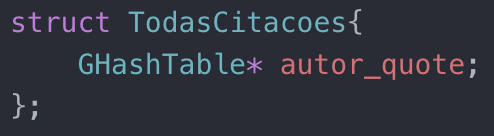
\includegraphics[scale=0.9]{TodasCitacoes.png}
\caption{Estrutura TodasCitacoes.}
\label{img:todas_citacoes}
\end{figure}

\begin{figure}[H]
\centering
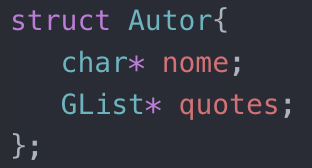
\includegraphics[scale=0.9]{Autor.png}
\caption{Estrutura Autor.}
\label{img:autor}
\end{figure}


\section{Alternativas, Decisões e Problemas de Implementação}
\subsection{Lista de Citações}


\subsection{Lista de Provérbios}


\subsection{Lista de Provérbios Adulterados}


\section{Testes realizados e Resultados}
\subsection{Lista de Citações}


\subsection{Lista de Provérbios}


\subsection{Lista de Provérbios Adulterados}


\chapter{Conclusão}
\label{chap:concl}


\end{document}
